\documentclass[../main/main.tex]{subfiles}

\raggedbottom

\makeatletter
\renewcommand{\@chapapp}{Chimie -- chapitre}
\makeatother

\begin{document}
\setcounter{chapter}{1}

\chapter{Transformation et \'equilibre chimique}

\section{Avancement d'une réaction}
\subsection{Présentation}
On considère la réaction de combustion du méthane~:
\[\ce{CH4\gaz{} + 2 O2\gaz{} = CO2\gaz{} + 2H2O\gaz}\]

Lorsqu'une molécule de méthane réagit, deux molécules de dioxygène sont
consommées et il se créé une molécule de dioxyde de carbone et une d'eau. Ainsi,
quand $\xi$ (se prononce «~ksi~») moles de $\ce{CH4}$ réagissent,
$2\xi$ moles de O$_2$ sont consommées pour augmenter de $\xi$ moles la quantité
de matière de CO$_2$ et de $2\xi$ moles celle de l'eau.

\begin{defi}[label=def:xi, sidebyside, righthand ratio=.3]{avancement molaire}
    La grandeur $\xi$ est appelée \textbf{avancement molaire de la réaction}, et
    elle permet de suivre l'évolution des quantités de matière des réactifs et
    des produis au cours d'une transformation chimique.
    \tcblower
    \tcbsubtitle[before skip=\baselineskip,
    colback=green!50!black,
    colframe=green!50!black]{Unités}
    $\xi$ est homogène à une quantité de matière et s'exprime en mol.
\end{defi}

On détermine cet avancement grâce à un tableau d'avancement, dont un exemple est
présenté ci-dessous~:

\begin{table}[tbh]
    \renewcommand{\arraystretch}{1.3}
    \centering
    \begin{tabularx}{\linewidth}{|p{3cm}||
        Y @{$+$} Y @{$\rightarrow$} Y @{$+$} Y |}\hline
        Équation     &
        ${\color{red}1}\ce{CH4\gaz{}} $&
        $\ce{{\color{orange}2}O2\gaz{}} $&
        ${\color{ForestGreen}1}\ce{CO2\gaz{}} $&
        $\ce{{\color{cornflowerblue}2}H2O\gaz{}}$
    \end{tabularx}
    \par\vspace{-\lineskip}%
    \begin{tabularx}{\linewidth}{|p{3cm}|| *4{Y|}}\hline
        État initial &
        $n_{\ce{CH4}}^0$ &
        $n_{\ce{O2}}^0 $ &
        $n_{\ce{CO2}}^0$ &
        $n_{\ce{H2O}}^0$ \\
        \hline
        En cours &
        $n_{\ce{CH4}}^0-{\color{red}1\xi} $&
        $n_{\ce{O2}}^0-{\color{orange}2\xi} $&
        $n_{\ce{CO2}}^0+{\color{ForestGreen}1\xi} $&
        $n_{\ce{H2O}}^0+{\color{cornflowerblue}2\xi} $\\
        \hline
    \end{tabularx}
\end{table}

\vspace{-12pt}
\begin{defi}[label=def:tabav]{tableau d'avancement}
    Le \textbf{tableau d'avancement} est l'outil central pour étudier une
    réaction chimique. Il est composé de 3 ou 4 lignes, comprenant
    \begin{enumerate}
        \item L'équation bilan, équilibrée grâce aux nombres stœchiométriques~;
        \item L'état initial de la réaction avec les quantités de matière des
            éléments~;
        \item L'état en cours de réaction avec l'évolution des $n$ déduite des
            nombres stœchiométriques~;
        \item L'état final de la réaction avec les quantités de matières à
            l'instant final.
    \end{enumerate}
\end{defi}

Quand on travaille à volume fixe, il peut être utile de travailler directement
avec les concentrations, donc avec $c_i = n_i/V$ avec $V$ le volume. On peut
donc définir l'avancement volumique~:

\begin{defi}[label=def:x, sidebyside, righthand ratio=.3]{avancement volumique}
    On définit $x$ l'\textbf{avancement volumique} de la réaction, tel que
    \[ \boxed{x = \frac{\xi}{V}}\]
    \tcblower
    \tcbsubtitle[before skip=\baselineskip,
    colback=green!50!black,
    colframe=green!50!black]{Unités}
    $x$ est homogène à une concentration et s'exprime en \si{mol.L^{-1}}.
\end{defi}

\subsection{Coefficients stœchiométriques algébriques}

Comme il est maintenant d'usage de le faire, on peut généraliser l'écriture
d'une réaction en faisant passer tous les termes d'un même côté. Par exemple,
pour la combustion du méthane~:
\[\ce{0 = CO2\gaz{} + 2H2O\gaz{} - CH4\gaz{} - 2O2\gaz{}}\]
Ceci fait apparaître les \textbf{coefficients stœchiométriques algébriques}, que
l'on note $\nu_i$ (se lit «~nu~»). Une équation bilan peut donc se mettre sous
la forme générale
\[ \boxed{\sum_i \nu_i\mathrm{X}_i = 0}\]
avec $\mathrm{X}_i$ les espèces intervenant dans la réaction. On a donc $\nu_i
>0$ si $\mathrm{X}_i$ est un produit, et $\nu_i < 0$ si c'est un réactif. Dans
l'exemple de la combustion du méthane, on a
\[ \begin{array}{rcl}
    \nu_{\ce{CH4}} = -1 \quad &\text{et}& \nu_{\ce{O2}}=-2\\
    \nu_{\ce{CO2}} = 1 \quad &\text{et}& \nu_{\ce{H20}}=2
\end{array}
\]

On peut donc généraliser la quantité de matière d'un composant directement avec
les coefficients algébriques~:
\[ \boxed{n_i = n_i^0 + \nu_i\xi}\]
avec $n_i$ la quantité de matière de l'élément $\mathrm{X}_i$, $n_i^0$ sa quantité
initiale et $\xi$ l'avancement.

\begin{instruc}[trans]{Transition}
    On peut trouver différents états finaux selon les propriétés des réactions
    et la composition initiale de celles-ci. Introduisons un peu de vocabulaire
    pour distinguer ces cas et les étudier.
\end{instruc}

\section{États d'équilibre et final d'un système chimique}
\subsection{Réactions totale et limitée}

\begin{defi}[label=def:final, sidebyside]
    {{avancement final et maximal, réactions totale et limitée}}
    À l'état final, quel qu'il soit, les quantités des matières sont données par
    l'\textbf{avancement final} $\xi_f$. L'avancement \textbf{maximal}
    $\xi_{\max}$ est l'avancement obtenu quand au moins un des réactifs est
    épuisé.
    \tcblower
    Quand $\xi_f = \xi_{\max}$, la réaction et alors \textbf{totale}. Sinon,
    elle est \textbf{limitée}. Une réaction totale se note avec un signe
    $\rightarrow$.
\end{defi}

Reprenons l'exemple initial, et déterminons l'avancement final en supposant que
l'on part avec
\[ n_{\ce{CH4}}^0 = \SI{2}{mol} \qet n_{\ce{O2}}^0 = \SI{3}{mol}\]
et que la réaction est totale. Pour trouver quel réactif et limitant, on cherche
quelle expression entre $n_{\ce{CH4}}^0-\xi $ et $n_{\ce{O2}}^0-2\xi $ donne
\textbf{le plus petit $\mathbf{\xi}$}. Si $\ce{CH4}$ est limitant, alors
$\xi_{\max} = \SI{2}{mol}$~; or, si $\ce{O2}$ est limiant, alors $\xi_{\max} =
\SI{1.5}{mol}$~: c'est donc le \textbf{dioxygène} qui est limitant, et
l'avancement maximal est de \SI{1.5}{mol}. On complète alors le tableau
d'avancement~:

\begin{center}
    \renewcommand{\arraystretch}{1.3}
    \centering
    \begin{tabularx}{\linewidth}{|p{3cm}||
        Y @{$+$} Y @{$\rightarrow$} Y @{$+$} Y |}\hline
        Équation     &
        $\ce{CH4\gaz{}} $ &
        $\ce{2O2\gaz{}}$ &
        $\ce{CO2\gaz{}}$ &
        $\ce{2H2O\gaz}$
    \end{tabularx}
    \par\vspace{-\lineskip}%
    \begin{tabularx}{\linewidth}{|p{3cm}|| *4{Y|}}\hline
        État initial (mol) &
        $2 $&
        $3 $&
        $0 $&
        $0 $\\
        \hline
        En cours (mol) &
        $2 -\xi$&
        $3 -2\xi$&
        $\xi$&
        $2\xi$\\
        \hline
        État final (mol) &
        $\num{0.5}$&
        $0$&
        $\num{1.5}$&
        $3$\\
        \hline
    \end{tabularx}
\end{center}

Il existe des situations où \textbf{tous les réactifs} sont limitant,
c'est-à-dire que l'avancement maximal met à $0$ toutes les quantités de matière
dans l'état final. On dit alors que les réactifs ont été introduits en
\textbf{proportions stœchiométriques}.

\begin{defi}[label=def:propsto]{proportions stœchiométriques}
    On dit que les réactifs ont été introduits dans des proportions
    stoechiométriques si les quantités de matière de tous les réactifs
    s'annulent si l'avancement était maximal.
\end{defi}

\begin{NCexem}[width=\linewidth, breakable]{Exercice}

    Lorsque l'on met du zinc solide dans un solution d'acide chlorhydrique, on
    observe un dégagement de dihydrogène et la formation d'ions zinc
    \ce{Zn^{2+}}. Le système initial est composé de \SI{0.11}{g} de zinc et
    d'une solution de \SI{20}{mL} d'acide chlorhydrique à \SI{5.0}{mol.L^{−1}}.
    \textbf{Déterminer le volume de dihydrogène formé}. Le volume molaire des
    gaz est \SI{24.5}{L.mol^{−1}}, et la masse molaire du zinc est $M(\ce{Zn}) =
    \SI{65.38}{g.mol^{-1}}$.
    \tcblower
    % Pour procéder, il faut dresser le tableau d'avancement et~:
    % \begin{enumerate}
    %     \item Écrire et équilibrer la réaction~;
    %     \item Déterminer les quantités initiales des réactifs~;
    %     \item Déterminer l'avancement maximal~;
    %     \item Conclure.
    % \end{enumerate}
    {\color{black}On traduit l'énoncé avec l'équation
    \[\boxed{\ce{Zn\sol + 2H+\aqu \rightarrow Zn^{2+}\aqu{} + H2\gaz{} }}\]
    Les quantités initiales de réactifs sont
    \[\boxed{n_{\ce{Zn}} = \frac{m}{M(\ce{Zn})} = \SI{1.68e-3}{mol}}
        \qet
    \boxed{n_{\ce{H+}} = [\ce{H+}]V = \SI{1.00e-1}{mol}}\]
    D'où le tableau
    \begin{center}
        \renewcommand{\arraystretch}{1.3}
        \centering
        \begin{tabularx}{\linewidth}{|p{4cm}||
            Y @{$+$} Y @{$\rightarrow$} Y @{$+$} Y  |}\hline
            Équation     &
            $\ce{Zn\sol} $ &
            $\ce{2H+\aqu}$ &
            $\ce{Zn^{2+}\aqu{}}$ &
            $\ce{H2\aqu{}}$
        \end{tabularx}
        \par\vspace{-\lineskip}%
        \begin{tabularx}{\linewidth}{|p{4cm}|| *4{Y|}}\hline
            État initial (mmol)&
            $1.68 $&
            $100 $&
            $0 $&
            $0 $\\
            \hline
            En cours (mmol)&
            $1.68 -\xi $&
            $100 -2\xi $&
            $\xi $&
            $\xi $\\
            \hline
            État final (mmol)&
            $0$&
            $\num{96.64}$ &
            $\num{1.68}$  &
            $\num{1.68}$ \\
            \hline
        \end{tabularx}
    \end{center}
    On trouve l'avancement maximal $\xi_{\max} = \SI{1.68e-3}{mol}$, et on
    obtient le volume de $\ce{H2\gaz{}}$ avec son volume molaire
    \[\boxed{V_{\ce{H2}} = n_{\ce{H2}}V_m = \SI{41}{mL}}\]}
\end{NCexem}

Une transformation limitée veut dire qu'il reste toujours un peu de réactif et
un peu de produit. Ceci est possible puisqu'il peut se produire la réaction
\begin{center}
    réactifs $\longrightarrow$ produits
\end{center}
mais dès que les produits sont présents, il peut aussi se passer
\begin{center}
    réactifs $\longleftarrow$ produits
\end{center}
On dit alors qu'il y a \textbf{équilibre chimique} lorsque les \textbf{deux
réactions ont des actions inverses l'une de l'autre}. On voit donc les écritures
suivantes~:
\[
    \boxed{\ce{\alpha_1R_1 + \alpha_2R_2} +…
        \xrightleftharpoons[\rm indirect]{\rm direct}
    \ce{\beta_1P_1 +\beta_2P_2} +…}
    \qou
    \boxed{\ce{\alpha_1R_1 + \alpha_2R_2} +…
            =
    \ce{\beta_1P_1 +\beta_2P_2}+…}
\]

\subsection{Quantifications de l'avancement}

Il y a d'autres grandeurs utilisées pour décrire l'avancement~:

\begin{defi}[label=def:tauxconvdissrendement, tabularx={Y|Y|Y}]
    {{Taux de conversion, coefficient de dissociation et rendement}}
    \textbf{Taux de conversion} &
    \textbf{Coefficient de dissociation} &
    \textbf{Rendement}\\\hline
    On définit le taux de conversion d'un réactif X$_i$ comme
    \[\boxed{\tau(t) = \frac{n_i^0 - n_i(t)}{n_i^0}}\]
    Il vaut 0 à $t=0$, et 1 s'il a complètement été consommé. &
    Le coefficient de dissociation $\alpha$ est le taux de conversion dans le
    cas où \textbf{seul un réactif} se dissocie. &
    Le rendement est le rapport entre l'avancement à un instant $t$ et
    l'avancement \textit{maximal} $\xi_{\max}$. On a
    \[\boxed{\eta = \frac{\xi}{\xi_{\max}}}\]
\end{defi}

\begin{instruc}[trans]{Transition}

    Nous cherchons donc un moyen de mettre en place des grandeurs pour
    déterminer le sens d'évolution d'un système en décrivant les actions des
    deux sens de la réaction.

\end{instruc}

\subsection{Quotient de réaction}

Pendant une réaction chimique, réactifs et produits s'opposent dans leur action
vis-à-vis de l'évolution du système.
Pour quantifier la tendance évolutive du l'équation, on fait appel aux
\textbf{activités} des éléments mis en jeu, \textit{via} une grandeur appelée
\textbf{quotient de réaction}.

\begin{defi}[label=quoreac]{Quotient de réaction}
    Soit une réaction
    \[\ce{\alpha_1R_1 + \alpha_2R_2} +…
            =
        \ce{\beta_1P_1 +\beta_2P_2}+…\]
    qui peut également s'écrire
    \[ \sum_i \nu_i\mathrm{X}_i = 0\]
    Le quotient de réaction $Q_r$ est alors
    \[\boxed{Q_r = \frac{a(\ce{P_1})^{\beta_1} \times
                         a(\ce{P_2})^{\beta_2} \times…}{
                         a(\ce{R_1})^{\alpha_1} \times
                         a(\ce{R_2})^{\alpha_2} \times…}}
      \qou
      \boxed{Q_r = \prod_i a(\ce{X_i})^{\nu_i}}
    \]
\end{defi}

\begin{exem}[label=exem:qr, sidebyside, righthand ratio=.45]{Exemples}
    Écrire les quotients de~:
    \begin{enumerate}
        \item $\ce{2I^-\aqu{} + S2O8^{2-}\aqu{} = I2\aqu{} +2SO4^{2-}\aqu}$
        \item $\ce{Ag+\aqu{} + Cl^-\aqu{} = AgCl\sol}$
        \item $\ce{2FeCl3\gaz{} = Fe2Cl6\gaz{}}$
    \end{enumerate}
    \tcblower{\color{black}
    ~\hspace{-12pt}
    \leftcenters{1)}{$\DS Q_r = \frac{[\ce{I2}]\times[\ce{SO4^{2-}}]^2}
            {[\ce{I-}]^2\times [\ce{S2O8^{2-}}]}$}\\
    \leftcenters{2)}{$\DS Q_r =
    \frac{c\degree^2}{[\ce{Ag+}]\times[\ce{Cl-}]}$}\\
    \leftcenters{3)}{$\DS Q_r = \frac{P_{\ce{Fe2Cl6}}/P\degree}
            {P_{\ce{FeCl3}}{}^2/P\degree{}^2} =
        P\degree\frac{P_{\ce{Fe2Cl6}}}{P_{\ce{FeCl3}}{}^2}$}
    }\vspace{-12pt}
\end{exem}

\subsection{Constante d'équilibre}
À l'équilibre chimique, les produits et réactifs se combinent dans des sens
opposés tout à fait équilibré. On définit donc la constante d'équilibre~:

\begin{defi}[label=def:K]{constante d'équilibre}
    À toute réaction chimique est associée une grandeura appelée
    \textbf{constante d'équilibre}, notée $K$, qui ne dépend que de la réaction
    considérée et de la température. Elle est égale au quotient réactionnel à
    l'équilibre chimique (état final)~:
    \[\boxed{K = Q_{r, f}}\]
    On l'appelle aussi la \textbf{relation de Guldberg-Waage} ou \textbf{loi
    d'action des masses}.
\end{defi}

Le quotient de réaction va évoluer de telle sorte à être égal à la constante de
réaction à l'équilibre~: celle-ci permet de déterminer l'état d'équilibre du
système, puisqu'elle donnera le lien entre les activités des composants à
l'avancement final et donc la composition du système.

On constate assez évidemment que la constante d'équilibre d'une réaction écrit
dans un sens est l'\textbf{inverse} de la constante d'équilibre de la même
réaction écrite dans l'autre sens.

\begin{NCexem}[width=\linewidth, breakable]{Exercice}
    Soit la réaction de l'acide éthanoïque avec l'eau~:
    \[\ce{CH3COOH\aqu{} + H2O\liq{} = CH3COO\moin{}\aqu{} + H3O\plus{}\aqu{}}\]
    de constante $K = \num{1.78e-5}$. On introduit $c = \SI{1.0e-1}{mol.L^{-1}}$
    d'acide éthanoïque et on note $V$ le volume de solution. Déterminer la
    composition à l'état final.
    \tcblower{\color{black}
    \begin{center}
        \renewcommand{\arraystretch}{1.3}
        \begin{tabularx}{\linewidth}{|p{3cm}||
            Y @{$+$} Y @{$=$} Y @{$+$} Y  |}\hline
            Équation     &
            $\ce{CH3COOH\aqu{}} $ &
            $\ce{H2O\liq{}}$ &
            $\ce{CH3COO\moin{}\aqu{}}$ &
            $\ce{H3O\plus{}\aqu{}}$
        \end{tabularx}
        \par\vspace{-\lineskip}%
        \begin{tabularx}{\linewidth}{|p{3cm}|| *4{Y|}}\hline
            État initial &
            $c $&
            excès&
            $0 $&
            $0 $\\
            \hline
            En cours &
            $c - x$&
            excès&
            $x $&
            $x $\\
            \hline
            État final &
            $c - x_f$&
            excès&
            $x_f $&
            $x_f $\\
            \hline
        \end{tabularx}
    \end{center}
    Par définition,
    \begin{gather*}
        K =
            \frac{[\ce{H3O\plus{}}]_f \times [\ce{CH3COO\moin{}}]_f}
            {c\degree[\ce{CH3COOH}]_f}
            =
            \frac{x_f{}^2}{c\degree(c-x_f)}\\
        \Leftrightarrow
        x_f{}^2 + Kc\degree x_f - cKc\degree = 0
    \end{gather*}
    On simplifie les calculs en ignorant $c\degree = \SI{1}{mol.L^{-1}}$. Ainsi
    ce polynôme a deux racines~:
    \begin{gather*}
        x_{f,1} = \frac{-K - \sqrt{K^2+4Kc}}{2}
        \qet
        x_{f,2} = \frac{-K + \sqrt{K^2+4Kc}}{2}\\
        x_{f,1} = \SI{-1.34e-3}{mol.L^{-1}}
        \qet
        x_{f,2} = \SI{1.32e-3}{mol.L^{-1}}
    \end{gather*}
    dont seule la seconde fait sens, étant donné qu'il n'y a pas de produit au
    départ~: on garde donc
    \[\boxed{x_f = \SI{1.32e-3}{mol.L^{-1}}}\]\vspace{-12pt}}
\end{NCexem}

Dans cet exemple, on pouvait effectuer une simplification en considérant la
valeur de la constante d'équilibre. En effet, le fait que la constante
d'équilibre soit petite veut dire l'équilibre va être atteint très vite, dès
qu'un peu des produits sont formés et que le ratio de leurs activités sur celles
des réactifs est égal à la constante d'équilibre. On a donc les propriétés
suivantes sur la constante d'équilibre~:

\begin{prop}[label=prop:K]{Constante d'équilibre et avancement} De manière
    qualitative, on a~:
    \begin{itemize}
        \item si $K < 1$, la réaction est favorisée dans le sens $\leftarrow$,
            et si $K < \num{e-4}$, alors la réaction est \textbf{peu avancée}
            dans le sens $\rightarrow$~;
        \item si $K > 1$, alors la réaction est favorisée dans le sens
            $\rightarrow$, et si $K > \num{e4}$, alors la réaction est
            \textbf{totale} (ou quasi-totale) dans le sens $\rightarrow$.
    \end{itemize}
\end{prop}

Ainsi, dans l'exercice précédent, on sait que $x \ll c$ puisque $K \ll
\num{e-4}$~: on peut donc écrire
\[ K = \frac{x_f{}^2}{c} \Leftrightarrow x_f = \sqrt{Kc} =
\SI{1.33e-3}{mol.L^{-1}}\]

\begin{instruc}[trans]{Transition}
    Comment la connaissance de l'équilibre d'un système peut-elle alors nous
    permettre de prédire son avancée~?
\end{instruc}

\section{Évolution d'un système chimique}
\subsection{Quotient réactionnel et sens d'évolution}

Étant donné que la constante d'équilibre est égale au quotient réactionnel à
l'équilibre, les activités des éléments chimiques vont évoluer de telle sorte à
ce que le quotient réactionnel atteigne l'équilibre~: s'il est inférieur à $K$
au départ, il doit augmenter au cours de la réaction et donc augmenter les
produits et réduire les réactifs, et inversement. On
retiendra

\begin{prop}[label=prop:qrsensevo]{sens d'évolution d'un système}
    \begin{itemize}
        \item Si $Q_r < K$, la réaction se déroule dans le sens direct~;
        \item Si $Q_r > K$, la réaction se déroule dans le sens indirect~;
    \end{itemize}
    \begin{center}
        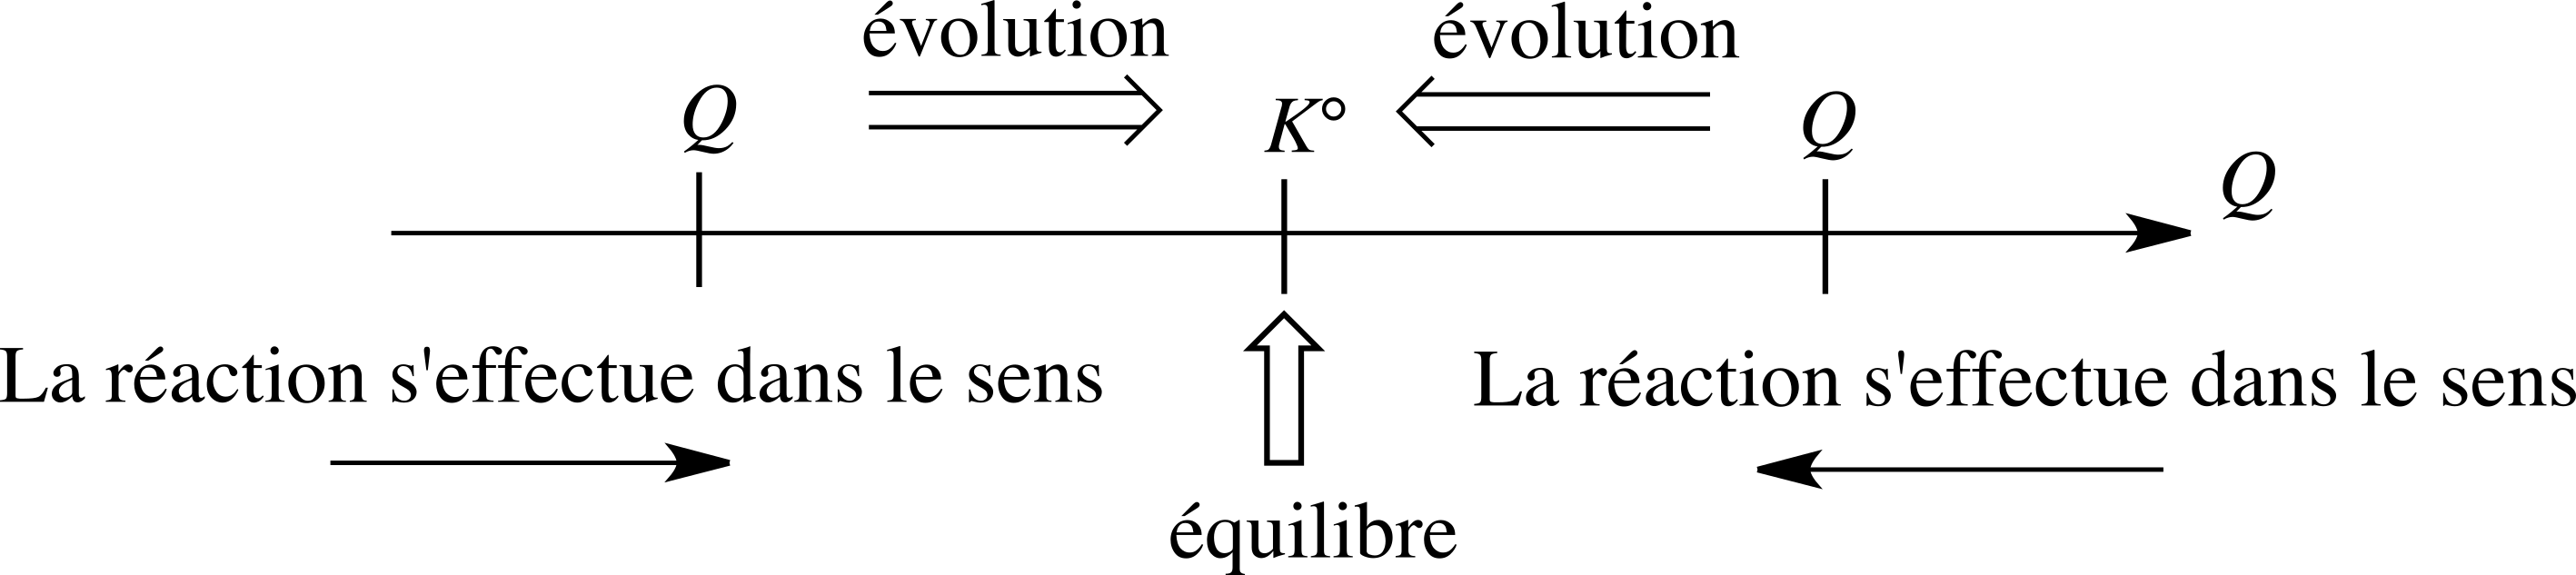
\includegraphics[width=.7\linewidth]{sensevo}
    \end{center}
\end{prop}

Prenons par exemple la réaction

\centersright{$\ce{Ag\plus{}\aqu{} + Cl\moin{}\aqu{} = AgCl\sol{}}$}{$K =
    \num{e9.7}$}

\begin{enumerate}
    \item Si $[\ce{Ag\plus{}}]_i = [\ce{Cl-}]_i = \SI{e-3}{mol.L^{-1}}$, alors
        \[Q_{r,i} = \frac{c\degree^2}{[\ce{Ag\plus{}}]_i \times [\ce{Cl-}]_i}
            = \num{e6} < K\]
        et la réaction se passe dans le sens direct~: on forme du précipité.
    \item Si $[\ce{Ag\plus{}}]_i = [\ce{Cl-}]_i = \SI{e-6}{mol.L^{-1}}$, alors
        \[Q_{r,i} = \frac{c\degree^2}{[\ce{Ag\plus{}}]_i \times [\ce{Cl-}]_i}
            = \num{e12} > K\]
        et la réaction se passe dans le sens indirect~: on dissout le précipité.
\end{enumerate}

\begin{NCexem}[width=\linewidth, breakable]{Exercice}
    Soit la synthèse de l'ammoniac~:

    \centersright{$\ce{N2\gaz{} + 3H2\gaz{} = 2NH3\gaz{}}$}{$K = \num{0.5}$}

    On introduit \SI{3}{mol} de diazote, \SI{5}{mol} de dihydrogène et
    \SI{2}{mol} d'ammoniac sous une pression de \SI{200}{bars}.
    \begin{enumerate}
        \item Déterminer les pressions partielles des gaz.
        \item Dans quel sens se produit la réaction~?
    \end{enumerate}
    \tcblower{\color{black}
    \begin{enumerate}
        \item Pour déterminer les pressions partielles, il nous faut la quantité
            de matière totale de gaz~: $n_{\rm tot} = 2+3+5 = \SI{10}{mol}$. On
            a donc
            \[p_{\ce{N2}} = x_{\ce{N2}}P = \SI{60}{bar}
              \quad
              p_{\ce{H2}} = x_{\ce{H2}}P = \SI{100}{bar}
              \quad
              p_{\ce{NH3}} = x_{\ce{NH3}}P = \SI{40}{bar}
          \]
        \item Pour connaître le sens de réaction, il faut le quotient
            réactionnel~:
            \[Q_r = \frac{p_{\ce{NH3}}{}^2\times p\degree^2}
                {p_{\ce{N2}}\times p_{\ce{H2}}{}^3} = \num{2.7e-5}
            \]
            Comme $Q_r < K$, la réaction se produit dans le sens
            \textbf{direct}~: on consomme $\ce{N2}$ et $\ce{H2}$ et on produit
            $\ce{NH3}$.
    \end{enumerate}\vspace{-15pt}}
\end{NCexem}

\begin{ror}[label=ror:gaz]{tableau avancement et gaz}
    On remarque que pour déterminer l'avancement d'une réaction avec des gaz, il
    faut avoir à tout instant la quantité de matière totale de gaz pour calculer
    les pressions partielles nécessaires au calcul de l'activité de chacun des
    gaz~: c'est pourquoi il est d'usage d'\textbf{ajouter une colonne $n_{\rm
    tot, gaz}$ dans les tableaux d'avancement}.
\end{ror}

Dans le cas de l'exercice précédent, on ferait donc~:

\begin{table}[h]
    \renewcommand{\arraystretch}{1.3}
    \centering
    \begin{tabularx}{\linewidth}{|p{3cm}||
        Y @{$+$} Y @{$=$} Y | M{3cm} |}\hline
        Équation     &
        $\ce{N2\gaz{}} $ &
        $\ce{3H2\gaz{}}$ &
        $\ce{2NH3\gaz{}}$ &
        $n_{\rm tot, gaz}$
    \end{tabularx}
    \par\vspace{-\lineskip}%
    \begin{tabularx}{\linewidth}{|p{3cm}|| *3{Y|} M{3cm}|}\hline
        État initial (mol)&
        $3 $&
        $5 $&
        $2 $&
        $10 $\\
        \hline
        En cours (mol) &
        $3 - \xi$&
        $5 - 3\xi$&
        $2 + 2\xi$&
        $10 - 2\xi$\\
        \hline
    \end{tabularx}
\end{table}

\subsection{Cas des ruptures d'équilibre}

Quand la réaction contient des solides ou liquides purs, les activités ne
peuvent pas évoluer, elles restent égales à 1. Dans ce cas, on peut arriver à ce
qu'on appelle une \textit{rupture d'équilibre}. Regardons la réaction de
dissolution du chlorure de sodium, de masse molaire $M(\ce{NaCl}) =
\SI{58.44}{g.mol^{-1}}$~:

\centersright{$\ce{NaCl\sol{} = Na\plus{}\aqu{} + Cl\moin{}\aqu{}}$}{$K=33$}

On introduit \SI{2.0}{g} de sel dans \SI{100}{mL} d'eau. Déterminons l'état
d'équilibre.\bigbreak

La quantité de matière introduite est
\[n = \frac{m}{M(\ce{NaCl})} = \SI{0.034}{mol}\]

\vspace{-15pt}
\begin{table}[h]
    \renewcommand{\arraystretch}{1.3}
    \centering
    \begin{tabularx}{\linewidth}{|p{3cm}||
        Y @{$=$} Y @{$+$} Y |}\hline
        Équation     &
        $\ce{NaCl\sol{}} $ &
        $\ce{Na\plus{}\aqu{}}$ &
        $\ce{Cl\moin{}\aqu{}}$
    \end{tabularx}
    \par\vspace{-\lineskip}%
    \begin{tabularx}{\linewidth}{|p{3cm}|| *3{Y|}}\hline
        État initial &
        $n $&
        $0 $&
        $0 $\\
        \hline
        État final &
        $n -\xi_f$&
        $\xi_f $&
        $\xi_f $\\
        \hline
    \end{tabularx}
\end{table}

La constante d'équilibre est
\begin{gather*}
    K = \frac{[\ce{Na+}]\times[\ce{Cl-}]}{c\degree^2}
      = \frac{1}{c\degree^2} \left(\frac{\xi_f}{V}\right)^2\\
    \Leftrightarrow
    \boxed{\xi_f = Vc\degree\sqrt{K} = \SI{0.57}{mol}}
\end{gather*}

Or, l'avancement maximal théorique est $\xi_{\max} = \SI{0.034}{mol} < \xi_f$~:
on ne peut donc pas atteindre l'équilibre, le solide est \textbf{dissout en
totalité}. On appelle ça une \textbf{rupture d'équilibre}.

\subsection{Résumé}

\begin{center}
    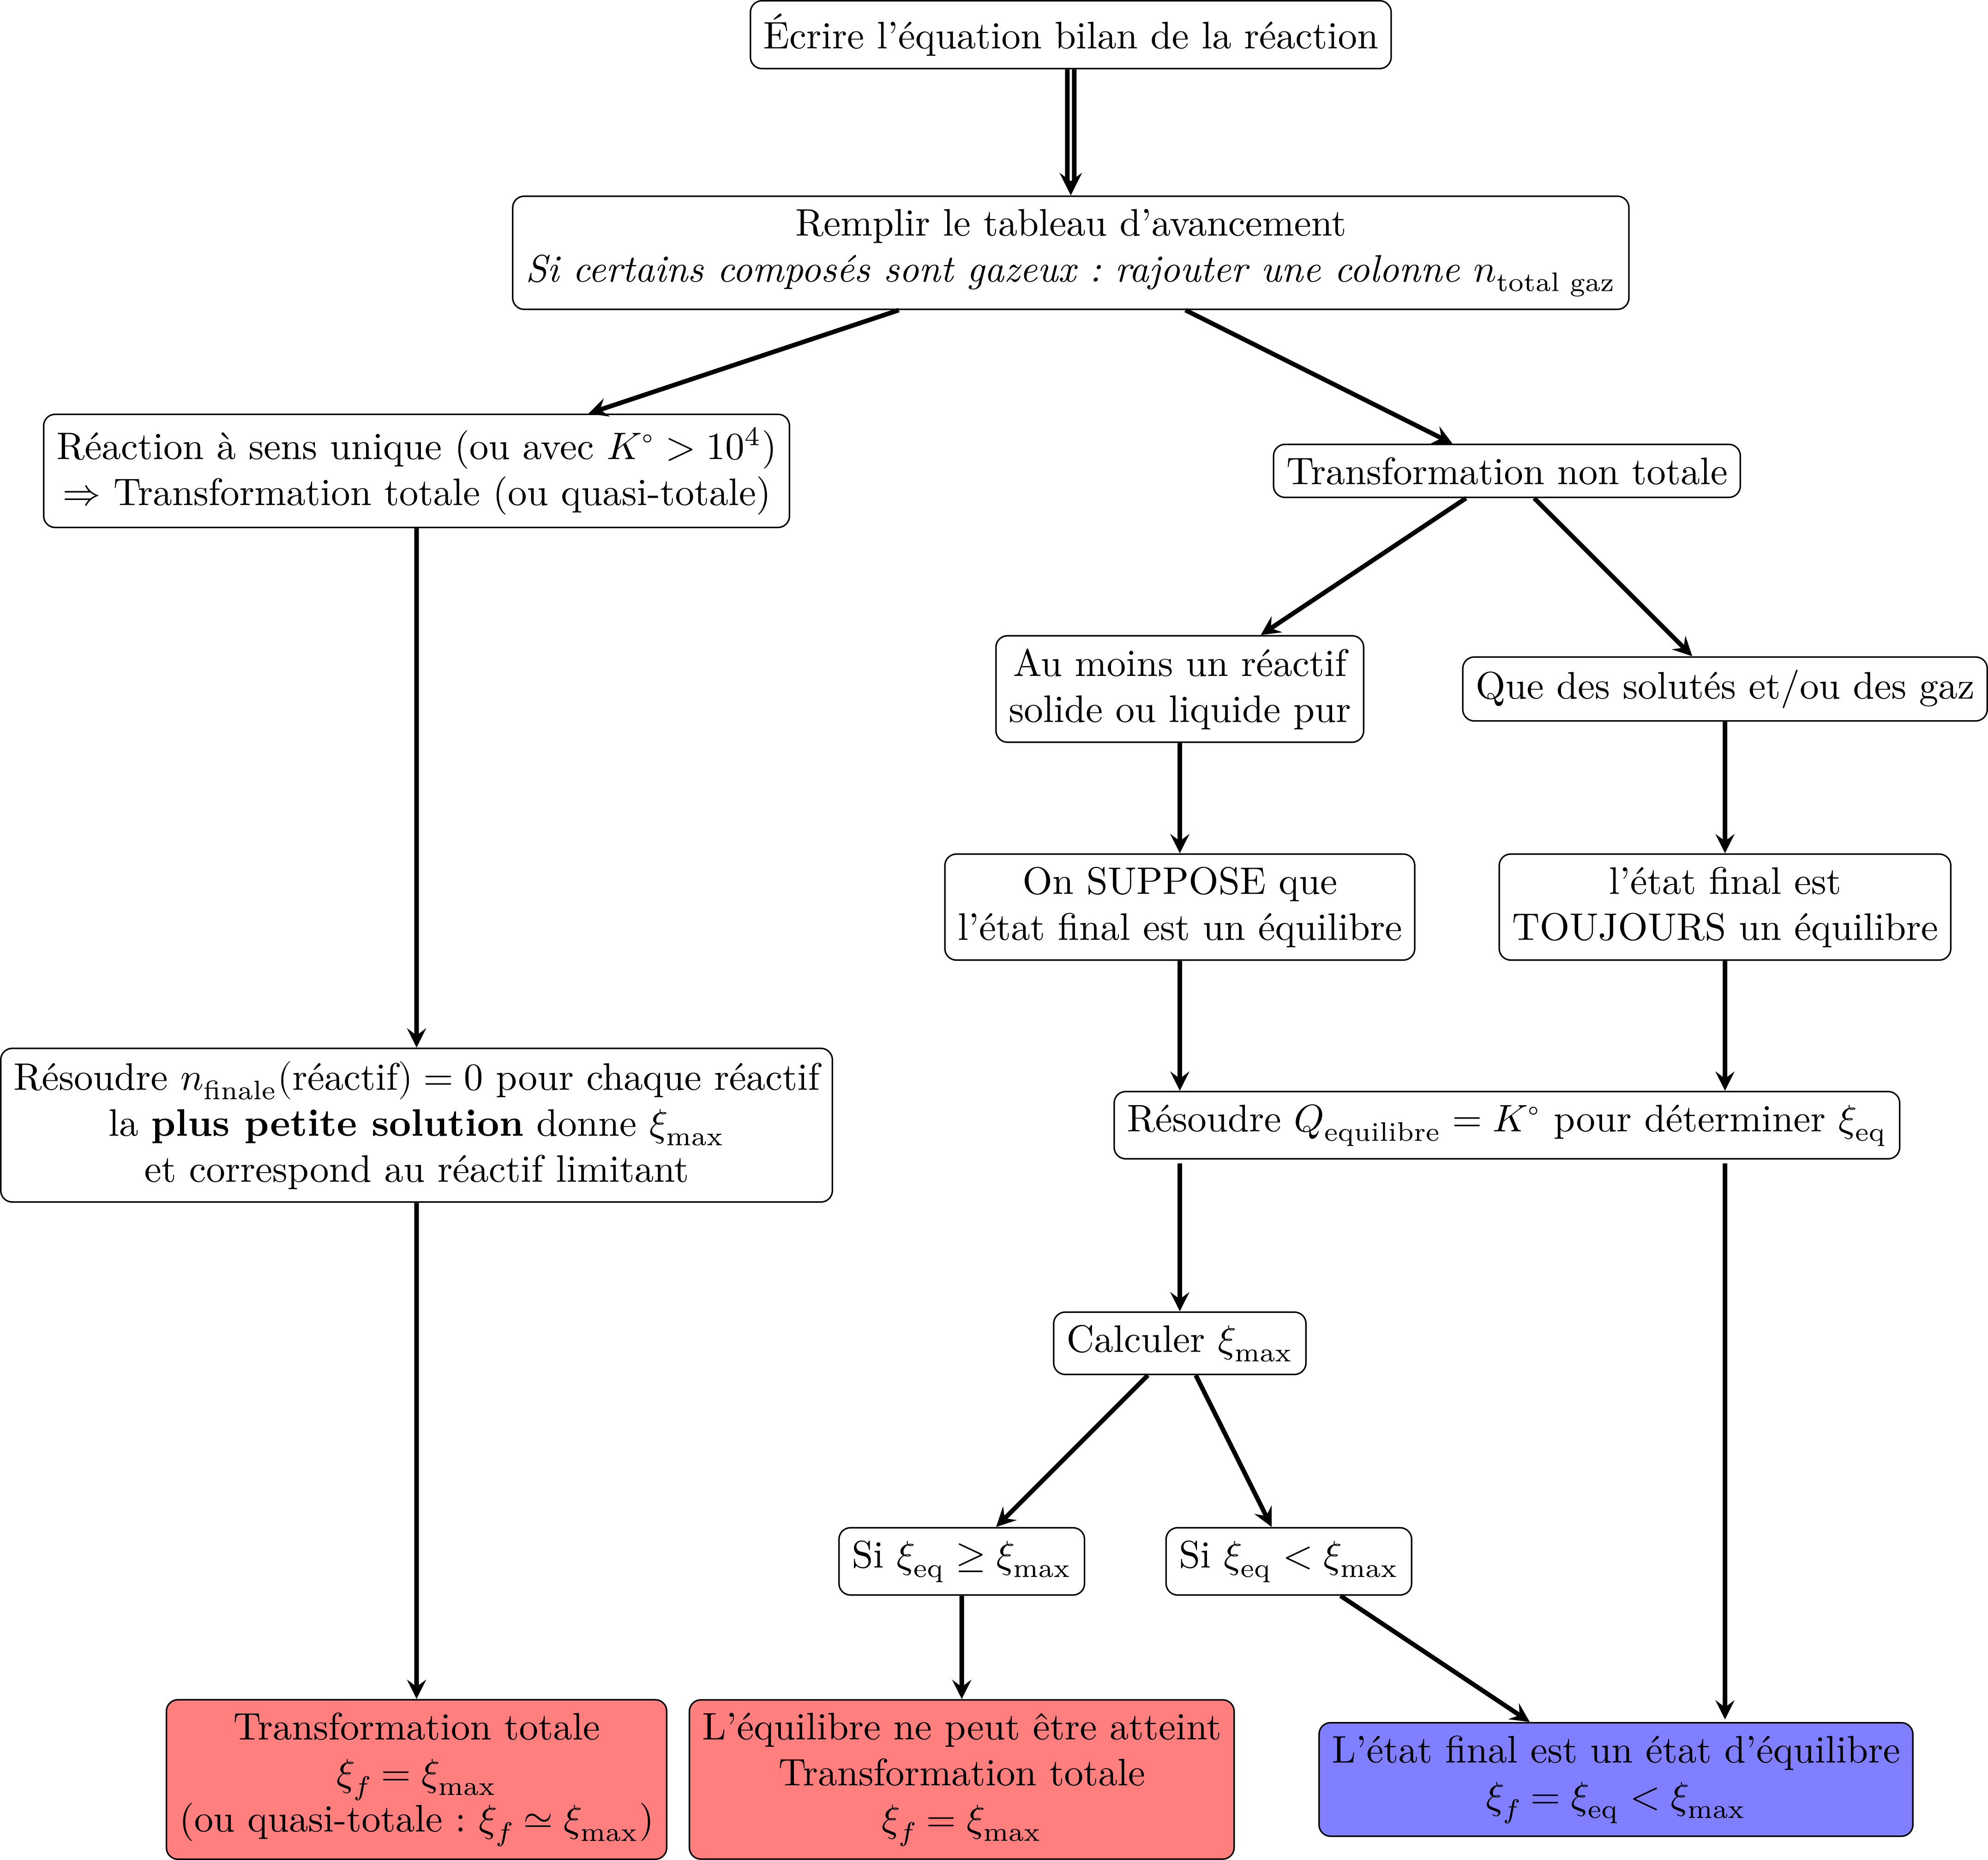
\includegraphics[width=\linewidth]{resume}
\end{center}
\end{document}
